% =====================================================================
%  HeartRateLab.jl — Print-ready TRI-FOLD A4 handout TEMPLATE
%  Structure / layout only — panel content is PLACEHOLDER, filled later.
%
%  Sheet:   A4 landscape, 297mm x 210mm, folded in thirds -> 6 panels.
%  Side 1 (page 1, "outer"): PANEL 1 Inner flap | PANEL 2 Back | PANEL 3 Front cover
%  Side 2 (page 2, "inner"): PANEL 4 Method | PANEL 5 Results  | PANEL 6 Feature table
%
%  Brand system copied from docs/poster/juliacon2026_poster.tex
%  (palette, card tcolorbox style, FiraSans, HRL + institutional logos).
%
%  Build:  pdflatex handout_trifold.tex   (run twice: QR + layout settle)
% =====================================================================
\documentclass[fontsize=9pt]{scrartcl}

\usepackage[T1]{fontenc}
\usepackage[utf8]{inputenc}
\usepackage[sfdefault]{FiraSans}
\usepackage[paperwidth=297mm,paperheight=210mm,margin=0mm]{geometry}
\usepackage{tikz}
\usetikzlibrary{calc,positioning,arrows.meta}
\usepackage[most]{tcolorbox}
\usepackage{qrcode}
\usepackage{graphicx}
\usepackage{array}
\usepackage{ragged2e}
\usepackage{fontawesome5}
\pagestyle{empty}
\setlength{\parindent}{0pt}
\renewcommand{\arraystretch}{1.35}

% ---------- JuliaCon / Julia brand palette (copied verbatim from the poster) ----------
\definecolor{jcindigo}{HTML}{38376C}   % primary bg
\definecolor{jcindigodk}{HTML}{201C46} % bg gradient bottom
\definecolor{jcpurple}{HTML}{4B518C}   % section rails
\definecolor{jclav}{HTML}{F3E8F2}      % light / footer band
\definecolor{jclavdk}{HTML}{D7D0DE}
\definecolor{jcgreen}{HTML}{389826}    % Julia green
\definecolor{jured}{HTML}{CB3C33}      % Julia red
\definecolor{jupurple}{HTML}{9558B2}   % Julia purple
\definecolor{jublue}{HTML}{4063D8}     % Julia blue
\definecolor{inkdark}{HTML}{23213F}

% ---------- fold geometry (A4 landscape, 297mm wide, letter/roll fold) ----------
% PANEL 1 (inner flap)   :   0mm ->  97mm   ( 97mm, narrower: the tuck-IN panel)
% PANEL 2 (back)         :  97mm -> 197mm   (100mm)
% PANEL 3 (front cover)  : 197mm -> 297mm   (100mm, outer wrap when folded)  % was: the panel
%                            that tucks INSIDE the other two when folded, so it
%                            is built ~3mm narrower to clear the crease without
%                            binding/buckling — standard roll-fold allowance)
\newlength{\panelA}\setlength{\panelA}{97mm}
\newlength{\panelB}\setlength{\panelB}{100mm}
\newlength{\panelC}\setlength{\panelC}{100mm}
% text-safe inset from each panel's true edges, keeps copy off the crease
\newlength{\safeLR}\setlength{\safeLR}{6mm}
\newlength{\safeTB}\setlength{\safeTB}{9mm}

% ---------- tcolorbox styles ----------
% full-height panel container (background colour only; no border/shadow —
% panels are edge-to-edge on the physical sheet, not floating cards)
\tcbset{
  panel/.style={enhanced, sharp corners, boxrule=0pt, valign=top, halign=left,
    left=\safeLR, right=\safeLR, top=\safeTB, bottom=\safeTB,
    before=\relax, after=\relax, before skip=0pt, after skip=0pt},
}
% brand "card" style — copied from the poster, padding scaled down for a
% ~85mm-wide handout column instead of an A0 poster column
\tcbset{
  card/.style={
    enhanced, colback=white, colframe=jcpurple,
    boxrule=0pt, arc=2.6mm, top=2.2mm, bottom=2.2mm, left=3.6mm, right=3.6mm,
    fontupper=\color{inkdark}\small,
    borderline west={2.2mm}{0mm}{jcgreen},
    drop fuzzy shadow=black!35,
  },
}
\newcommand{\ctitle}[2][jcgreen]{{\color{#1}\bfseries\large #2}\par\vspace{1.6mm}}
% small pill label used on every panel: "PANEL N — description"
\newcommand{\panellabel}[2][jcgreen]{%
  {\setlength{\fboxsep}{2.6pt}\colorbox{#1}{\color{white}\bfseries\footnotesize\ PANEL~#2\ }}\par\vspace{2.2mm}}
% dashed placeholder box, stands in for a figure/photo that will be dropped in later
\newcommand{\figph}[2]{%
  \tikz{\node[draw=gray!70,dashed,line width=0.6pt,rounded corners=1.5mm,
    align=center,text width=#1-4mm,minimum height=#2,inner sep=2mm,
    font=\footnotesize\itshape,text=gray!70]{[FIGURE PLACEHOLDER]\\ #1 $\times$ #2};}}
% Julia dots wordmark (from the poster)
\newcommand{\juliadots}[1]{%
\begin{tikzpicture}[scale=#1]
  \fill[jcgreen]  (0,0.52) circle (0.3);
  \fill[jublue]   (-0.45,0) circle (0.3);
  \fill[jured]    (0,0) circle (0.3);
  \fill[jupurple] (0.45,0) circle (0.3);
\end{tikzpicture}}

% ---------- fold-guide overlay: dashed crease lines + FOLD tabs ----------
% Purely a working-template aid (cut/fold registration); drop this block for
% camera-ready art once print bleed/trim is finalised with the print shop.
\newcommand{\foldguides}{%
\begin{tikzpicture}[remember picture,overlay]
  \foreach \x in {97mm,197mm}{
    \draw[gray!55,dash pattern=on 2pt off 2pt,line width=0.5pt]
      ($(current page.south west)+(\x,0)$) -- ($(current page.north west)+(\x,0)$);
    \node[fill=white,fill opacity=0.85,text opacity=1,draw=gray!55,line width=0.4pt,
          font=\tiny\bfseries,inner sep=1.2pt,rounded corners=0.8pt]
      at ($(current page.north west)+(\x,-3.2mm)$) {FOLD};
    \node[fill=white,fill opacity=0.85,text opacity=1,draw=gray!55,line width=0.4pt,
          font=\tiny\bfseries,inner sep=1.2pt,rounded corners=0.8pt]
      at ($(current page.south west)+(\x,3.2mm)$) {FOLD};
  }
\end{tikzpicture}}

\begin{document}

% =====================================================================
%  SIDE 1 — OUTER (what you see before/while folded)
%  left-to-right on the flat sheet: PANEL 1 Inner flap | PANEL 2 Back | PANEL 3 Front cover
% =====================================================================
\noindent%
\begin{minipage}[t][210mm][t]{\panelA}%
\begin{tcolorbox}[panel,colback=jcindigodk,width=\panelA,height=210mm,fontupper=\color{white}]
  \vspace{5mm}
  {\raggedright\color{white}\bfseries\fontsize{17}{21}\selectfont
   Feature selection:\\[0.5mm] meditation vs normal\par}
  \vspace{7mm}

  {\color{jclav}\bfseries\normalsize The collinearity problem\par}\vspace{2mm}
  {\raggedright\normalsize\color{white!90}
   Many HRV features are, by definition, functions of others, so the method must
   not treat them as independent evidence. On the healthy reference:\par}
  \vspace{1.6mm}
  {\raggedright\normalsize\color{white!90}
   \textbullet~$\mathrm{SD1}\equiv\mathrm{RMSSD}\equiv\mathrm{SDSD}$ ($|r|=1.00$)\par
   \vspace{1mm}
   \textbullet~$\mathrm{LF\,\%}\equiv\mathrm{LF\text{-}rel}$,\;
     $\mathrm{HF\,\%}\equiv\mathrm{HF\text{-}rel}$\par
   \vspace{1mm}
   \textbullet~$\mathrm{SDNN}\approx\mathrm{SD2}$ (0.98);\;
     Mean\,$\approx$\,Median IBI (1.00)\par}
  \vspace{7mm}

  {\color{jclav}\bfseries\normalsize The model\par}\vspace{2mm}
  {\raggedright\normalsize\color{white!90}
   \textbf{L1-regularized logistic regression} (meditation-state vs healthy),
   standardized to the healthy frame, solved by proximal-gradient \textbf{FISTA}.
   L1 keeps one representative of each collinear cluster and drops the rest --- the
   model de-duplicates for us.\par}
  \vspace{2.5mm}
  {\raggedright\normalsize\color{white!90}
   Instead of one fit, \textbf{stability selection}: \textbf{200 resamples}, each
   drawing meditation \emph{records} and healthy \emph{subjects} as whole groups
   (windows never leak across a split), classes balanced. We report how often each
   feature is selected.\par}
  \vspace{7mm}

  {\color{jclav}\bfseries\normalsize Most-stably selected\par}\vspace{2mm}
  {\color{white!92}\normalsize
   \renewcommand{\arraystretch}{1.3}\setlength{\tabcolsep}{4pt}%
   \begin{tabular}{@{}l r c@{}}
     \textbf{Feature} & \textbf{stability} & \textbf{dir}\\ \hline
     LF/HF & 77\,\% & $\uparrow$\\
     HF peak & 70\,\% & $\uparrow$\\
     LF rel / LF \% & 67\,\% & $\uparrow$\\
     LF peak & 64\,\% & $\uparrow$\\
     pNN20 & 61\,\% & $\uparrow$\\
     Total power & 52\,\% & $\uparrow$\\
     LF power & 47\,\% & $\uparrow$\\
   \end{tabular}\par}
  \vspace{4mm}
  {\raggedright\normalsize\color{white!90}
   Subject-grouped 5-fold CV \textbf{AUC $=0.73\pm0.27$}. The model most stably
   selects the \textbf{$\sim$0.1\,Hz LF-band} features ($+$pNN20) --- coherent with
   the slow $\sim$6\,breaths/min pacing of Chi \& Kundalini meditation. \textbf{The
   LF-band story the poster tells, earned by selection rather than asserted} --- but
   modest: no feature above 77\,\%, only \textbf{11 meditators}; exploratory, not a
   validated classifier.\par}
\end{tcolorbox}%
\end{minipage}%
\begin{minipage}[t][210mm][t]{\panelB}%
\begin{tcolorbox}[panel,colback=jclav,width=\panelB,height=210mm]
  \vspace{10mm}

  
\includegraphics[width=74mm]{figs/hrl_logo_side_dark.png}\par
  \vspace{7mm}
  {\raggedright\color{inkdark}\normalsize
   \textbf{The data behind the poster.} Every number, prior and longitudinal
   plot that would not fit on the A0 sheet --- the exact z-score table, the
   fitted scoring families, the selection model, and P1's own correlation.\par}
  \vspace{20mm}

  {\normalsize\bfseries\color{jcpurple} Institutional support\par}\vspace{4mm}
  
\includegraphics[height=12mm]{figs/inst_lasalle.png}\hspace{5mm}
  
\includegraphics[height=12mm]{figs/inst_tu.png}\hspace{5mm}
  
\includegraphics[height=12mm]{figs/inst_mu.pdf}\par
  \vspace{20mm}

  {\normalsize\bfseries\color{jcpurple} Author\par}\vspace{2.5mm}
  {\large\color{inkdark} Luis Alberto Barradas Chac\'on\par}
  {\normalsize\color{inkdark} TU Graz \textperiodcentered{} Med Uni Graz\par}
  \vspace{7mm}
  {\normalsize\bfseries\color{jured} MIT licence \textperiodcentered{} Open data \textperiodcentered{} Open source}\par
  \vspace{2.5mm}
  {\normalsize\faGithub~abcsds/HeartRateLab.jl\par}
  \vspace{9mm}\vfill

  % juliacon-style footer, condensed for the back panel
  \juliadots{0.6}\hspace{2mm}%
  {\color{inkdark}\bfseries\LARGE julia}{\color{jupurple}\bfseries\LARGE con}%
  \hspace{2mm}{\color{inkdark}\bfseries\normalsize Global~\textcolor{jublue}{\textbullet}~2026}\par
  \vspace{2.5mm}
  {\normalsize\color{jured}\bfseries Mainz, Germany \textperiodcentered{} Aug 10--15, 2026}\par
  {\small\color{jcpurple}Supplementary data sheet \textperiodcentered{} Julia 1.11}
\end{tcolorbox}%
\end{minipage}%
\begin{minipage}[t][210mm][t]{\panelC}%
\begin{tcolorbox}[panel,colback=jcindigo,width=\panelC,height=210mm,fontupper=\color{white}]
  \vspace{20mm}

  \begin{center}
    
\includegraphics[width=84mm]{figs/hrl_logo_side_white.png}\par
    \vspace{16mm}
    {\color{white}\bfseries\fontsize{28}{32}\selectfont HeartRateLab.jl}\par
    \vspace{4mm}
    {\color{jclav}\LARGE The data \& receipts behind the poster}\par
    \vspace{20mm}

    {\color{white}\bfseries\fontsize{19}{24}\selectfont
     Is this new experimental\\[1.5mm] data \emph{normal}?}\par
    \vspace{18mm}

    \begin{tcolorbox}[enhanced,colback=white,colframe=white,boxrule=0pt,arc=3mm,
         width=48mm,height=48mm,halign=center,valign=center,left=2mm,right=2mm,top=2mm,bottom=2mm]
       \qrcode[height=42mm]{https://s.barcha.xyz/juliacon2026-poster}
    \end{tcolorbox}\par
    \vspace{4mm}
    {\normalsize\color{white!85} albertobarradas.com}
  \end{center}
  \vfill
  \begin{center}
  {\small\color{white!75} Luis Alberto Barradas Chac\'on \textperiodcentered{} TU Graz \textperiodcentered{} Med Uni Graz}
  \end{center}
\end{tcolorbox}%
\end{minipage}%
\foldguides

\newpage

% =====================================================================
%  SIDE 2 — INNER (revealed once unfolded)
%  Printed on the reverse with a TOP-EDGE (short-edge) duplex flip, so panel
%  N on this side sits physically directly behind panel N on side 1 — i.e.
%  Panel 4 is behind Panel 1, Panel 5 behind Panel 2, Panel 6 behind Panel 3.
%  Column widths therefore repeat 100mm | 100mm | 97mm left-to-right.
% =====================================================================
\noindent%
\begin{minipage}[t][210mm][t]{\panelA}%
\begin{tcolorbox}[panel,colback=jcindigodk,width=\panelA,height=210mm,fontupper=\color{white}]
  \vspace{3mm}

  \begin{tcolorbox}[card, borderline west={2.2mm}{0mm}{jcgreen}]
    \ctitle[jcgreen]{Scoring families \& goodness of fit}
    {\color{inkdark}\footnotesize
     The normative prior fitted to each scored feature (MLE over
     61{,}715 healthy windows), with its parameters and KS $p$.\par}
    \vspace{1.6mm}
    {\color{inkdark}\footnotesize
    \renewcommand{\arraystretch}{1.28}%
    \setlength{\tabcolsep}{3.2pt}%
    \begin{tabular}{@{}l l l r@{}}
      \textbf{Feature} & \textbf{Family} & \textbf{Params} & \textbf{KS $p$}\\
      \hline
      LF/HF & LogN & $0.852,\,0.869$ & $7\mathrm{e}{-9}$\\
      LF power & Gamma & $0.868,\,705$ & $5\mathrm{e}{-118}$\\
      TINN & Gamma & $5.32,\,30.9$ & $2\mathrm{e}{-18}$\\
      Total power & Gamma & $0.946,\,1650$ & $2\mathrm{e}{-125}$\\
      HRV tri-index & Gamma & $5.94,\,1.74$ & $1\mathrm{e}{-14}$\\
      LF rel & Beta & $5.13,\,8.02$ & $2\mathrm{e}{-12}$\\
      LF \% & Gamma & $8.66,\,4.50$ & $3\mathrm{e}{-4}$\\
      cCSI & LogN & $6.64,\,0.882$ & $4\mathrm{e}{-5}$\\
      SD2 & Gamma & $3.73,\,18.7$ & $2\mathrm{e}{-24}$\\
      SD2/SD1 & LogN & $1.14,\,0.533$ & $1\mathrm{e}{-7}$\\
      SDNN & Gamma & $3.79,\,14.0$ & $4\mathrm{e}{-29}$\\
      SD1$\cdot$SD2 area & LogN & $8.21,\,1.01$ & $7\mathrm{e}{-16}$\\
      CVI & Normal & $4.27,\,0.439$ & $7\mathrm{e}{-16}$\\
      pNN20 & Beta & $1.81,\,3.30$ & $2\mathrm{e}{-17}$\\
      pNN50 & Beta & $0.321,\,3.56$ & $2\mathrm{e}{-98}$\\
      rRR & Gamma & $4.16,\,0.881$ & $3\mathrm{e}{-172}$\\
      IBI range & Gamma & $3.49,\,94.1$ & $4\mathrm{e}{-14}$\\
      Max IBI & Normal & $953,\,197$ & $3\mathrm{e}{-11}$\\
      Mean IBI & Normal & $780,\,147$ & $1\mathrm{e}{-64}$\\
      Min IBI & Normal & $625,\,128$ & $5\mathrm{e}{-27}$\\
      Median IBI & Normal & $780,\,151$ & $1\mathrm{e}{-77}$\\
      CVSD & Gamma & $2.93,\,0.0146$ & $6\mathrm{e}{-44}$\\
      RMSSD & Gamma & $2.40,\,14.2$ & $3\mathrm{e}{-50}$\\
      SD1 & Gamma & $2.40,\,10.1$ & $3\mathrm{e}{-50}$\\
      SDSD & Gamma & $2.40,\,14.2$ & $3\mathrm{e}{-50}$\\
      LF peak & Normal & $0.0642,\,0.0183$ & $3\mathrm{e}{-306}$\\
      sdann & Gamma & $0.873,\,27.8$ & $6\mathrm{e}{-28}$\\
      HF power & Gamma & $0.615,\,587$ & $7\mathrm{e}{-208}$\\
      Min HR & Normal & $100,\,21.1$ & $1\mathrm{e}{-40}$\\
      Mean HR & Normal & $79.7,\,15.2$ & $2\mathrm{e}{-95}$\\
      Max HR & Normal & $65.7,\,13.8$ & $9\mathrm{e}{-68}$\\
      HF peak & Normal & $0.213,\,0.0633$ & $1\mathrm{e}{-111}$\\
      SD HR & Gamma & $3.79,\,392$ & $1\mathrm{e}{-9}$\\
      HF rel & Beta & $1.31,\,5.44$ & $3\mathrm{e}{-40}$\\
      HF \% & Gamma & $2.48,\,7.84$ & $1\mathrm{e}{-26}$\\
    \end{tabular}\par}
    \vspace{1.6mm}
    {\footnotesize\color{jcpurple}\itshape KS-rejected at $n\approx62$k --- these
     are convenient scoring families, not fitted laws; read $z$ descriptively.
     Full 53-feature registry at github.com/abcsds/HeartRateLab.jl.\par}
  \end{tcolorbox}
\end{tcolorbox}%
\end{minipage}%
\begin{minipage}[t][210mm][t]{\panelB}%
\begin{tcolorbox}[panel,colback=jcindigo,width=\panelB,height=210mm,fontupper=\color{white}]
  \vspace{3mm}

  \begin{tcolorbox}[card, borderline west={2.2mm}{0mm}{jupurple}]
    \ctitle[jupurple]{P1: all 35 scored features}
    {\color{inkdark}\footnotesize
     P1's window-median value and its $z$ against each reference; $z$ is a
     per-window descriptive percentile. Sorted by $z$ vs healthy.\par}
    \vspace{1.6mm}
    {\color{inkdark}\scriptsize
    \renewcommand{\arraystretch}{1.0}%
    \setlength{\tabcolsep}{2.6pt}%
    \begin{tabular}{@{}l r r r@{}}
      \textbf{Feature} & \textbf{P1 val} & \textbf{$z$ heal.} & \textbf{$z$ med.}\\
      \hline
      \textbf{LF/HF} & $\mathbf{22.8}$ & $\mathbf{+2.6}$ & $\mathbf{+1.7}$\\
      LF power & $3461$ & $+2.6$ & $+0.9$\\
      TINN & $320$ & $+1.9$ & $+1.2$\\
      Total power & $5422$ & $+1.8$ & $+0.6$\\
      HRV tri-index & $17.1$ & $+1.5$ & $+1.0$\\
      LF rel & $0.583$ & $+1.4$ & $+0.6$\\
      LF \% & $58.3$ & $+1.4$ & $+0.7$\\
      cCSI & $2453$ & $+1.3$ & $+1.2$\\
      SD2 & $112$ & $+1.2$ & $+0.7$\\
      SD2/SD1 & $5.54$ & $+1.1$ & $+1.2$\\
      SDNN & $81.5$ & $+1.1$ & $+0.5$\\
      SD1$\cdot$SD2 area & $8010$ & $+0.8$ & $+0.1$\\
      CVI & $4.61$ & $+0.8$ & $+0.1$\\
      \textbf{pNN20} & $\mathbf{0.492}$ & $\mathbf{+0.7}$ & $\mathbf{+2.6}$\\
      pNN50 & $0.072$ & $+0.4$ & $+0.2$\\
      rRR & $3.86$ & $+0.3$ & $-0.4$\\
      IBI range & $340$ & $+0.2$ & $-0.1$\\
      Max IBI & $980$ & $+0.1$ & $-0.1$\\
      Mean IBI & $788$ & $+0.1$ & $+0.1$\\
      Min IBI & $626$ & $0.0$ & $+0.1$\\
      Median IBI & $782$ & $0.0$ & $+0.1$\\
      CVSD & $0.038$ & $0.0$ & $-0.5$\\
      RMSSD & $29.4$ & $0.0$ & $-0.5$\\
      SD1 & $20.8$ & $0.0$ & $-0.5$\\
      SDSD & $29.4$ & $0.0$ & $-0.5$\\
      LF peak & $0.064$ & $0.0$ & $-0.2$\\
      sdann & $15.2$ & $0.0$ & $-0.1$\\
      HF power & $143$ & $-0.2$ & $-0.7$\\
      Min HR & $95.8$ & $-0.2$ & $-0.2$\\
      Mean HR & $76.1$ & $-0.2$ & $-0.3$\\
      Max HR & $61.2$ & $-0.3$ & $-0.1$\\
      HF peak & $0.167$ & $-0.7$ & $-0.5$\\
      SD HR & $736$ & $-1.0$ & $-0.6$\\
      HF rel & $0.027$ & $-1.5$ & $-1.1$\\
      HF \% & $2.72$ & $-2.1$ & $-1.5$\\
    \end{tabular}\par}
    \vspace{1.6mm}
    {\footnotesize\color{jcpurple}\itshape All 35 scored features; $z$ is a
     per-window descriptive percentile, not an inferential test. Redundant rows
     (SD1$\equiv$RMSSD$\equiv$SDSD, LF\,\%$\equiv$LF-rel) are handled by the
     selection model --- never read them as independent evidence.\par}
  \end{tcolorbox}
  \vspace{2.5mm}

  \begin{tcolorbox}[card, borderline west={2.2mm}{0mm}{jublue}]
    \ctitle[jublue]{Breathing rate $=$ frequency: why P1's LF is high}
    {\color{inkdark}\footnotesize
     A breathing rate maps to a spectral frequency ($\mathrm{Hz}=\mathrm{BPM}/60$);
     \textbf{every} rate below lands inside the \textbf{LF band} (0.04--0.15\,Hz),
     and resonant $\sim$6/min sits at its 0.1\,Hz centre.\par}
    \vspace{1.6mm}
    {\color{inkdark}\footnotesize
    \renewcommand{\arraystretch}{1.05}\setlength{\tabcolsep}{5pt}%
    \begin{tabular}{@{}r r r@{}}
      \textbf{Breaths/min} & \textbf{Cycle (s)} & \textbf{Freq (Hz)}\\
      \hline
      $3.5$ & $17.1$ & $0.058$\\
      $4.0$ & $15.0$ & $0.067$\\
      $4.5$ & $13.3$ & $0.075$\\
      $5.0$ & $12.0$ & $0.083$\\
      $5.5$ & $10.9$ & $0.092$\\
      $\mathbf{6.0}$ & $\mathbf{10.0}$ & $\mathbf{0.100}$\\
      $6.5$ & $9.2$ & $0.108$\\
      $7.0$ & $8.6$ & $0.117$\\
      $7.5$ & $8.0$ & $0.125$\\
      $8.0$ & $7.5$ & $0.133$\\
      $8.5$ & $7.1$ & $0.142$\\
      $9.0$ & $6.7$ & $0.150$\\
    \end{tabular}\par}
    \vspace{1.4mm}
    {\footnotesize\color{jublue}\itshape \textbf{Bold} row = resonant $\sim$6/min
     $=$ 0.1\,Hz, the LF-band centre.\par}
  \end{tcolorbox}
\end{tcolorbox}%
\end{minipage}%
\begin{minipage}[t][210mm][t]{\panelC}%
\begin{tcolorbox}[panel,colback=jcindigo,width=\panelC,height=210mm,fontupper=\color{white}]
  \vspace{3mm}

  \begin{tcolorbox}[card, borderline west={2.2mm}{0mm}{jured}]
    \ctitle[jured]{Meditators vs the normal population}
    {\color{inkdark}\footnotesize
     The meditation cohort ($n=11$, during-meditation) scored against the healthy
     prior --- quantile $z$ per feature. \textbf{Positive = higher than the general
     population.}\par}
    \vspace{1.6mm}
    {\color{inkdark}\scriptsize
    \renewcommand{\arraystretch}{1.0}%
    \setlength{\tabcolsep}{2.6pt}%
    \begin{tabular}{@{}l r @{\hspace{5mm}} l r@{}}
      \textbf{Feature} & \textbf{$z$} & \textbf{Feature} & \textbf{$z$}\\
      \hline
      \textbf{LF power} & $\mathbf{+1.2}$ & CVSD & $+0.3$\\
      \textbf{LF/HF} & $\mathbf{+1.0}$ & HF power & $+0.3$\\
      LF \% & $+0.9$ & SD2/SD1 & $+0.3$\\
      LF rel & $+0.9$ & Max IBI & $+0.2$\\
      Total power & $+0.9$ & Mean IBI & $+0.2$\\
      CVI & $+0.8$ & Median IBI & $+0.2$\\
      SD1$\cdot$SD2 area & $+0.8$ & sdann & $+0.2$\\
      SDNN & $+0.8$ & Min IBI & $+0.1$\\
      SD2 & $+0.7$ & LF peak & $-0.1$\\
      rRR & $+0.6$ & Min HR & $-0.3$\\
      HRV tri-index & $+0.6$ & Mean HR & $-0.4$\\
      cCSI & $+0.4$ & Max HR & $-0.4$\\
      TINN & $+0.4$ & pNN20 & $-0.4$\\
      pNN50 & $+0.4$ & HF rel & $-0.5$\\
      SDSD & $+0.3$ & HF peak & $-0.7$\\
      SD1 & $+0.3$ & HF \% & $-0.7$\\
      RMSSD & $+0.3$ & SD HR & $-0.8$\\
      IBI range & $+0.3$ & &\\
    \end{tabular}\par}
    \vspace{1.6mm}
    {\footnotesize\color{jured}\itshape A mild but coherent shift \textbf{into the LF
     band} (LF power $+1.2$, LF/HF $+1.0$) with vagal tone barely moved --- the same
     direction as P1, which is why P1 reads \textbf{meditator-like}. The meditators
     are a reference group, not the finding.\par}
  \end{tcolorbox}
  \vspace{3mm}

  {\color{jclav}\bfseries\small P1's own feature correlation\par}\vspace{1.5mm}
  \begin{center}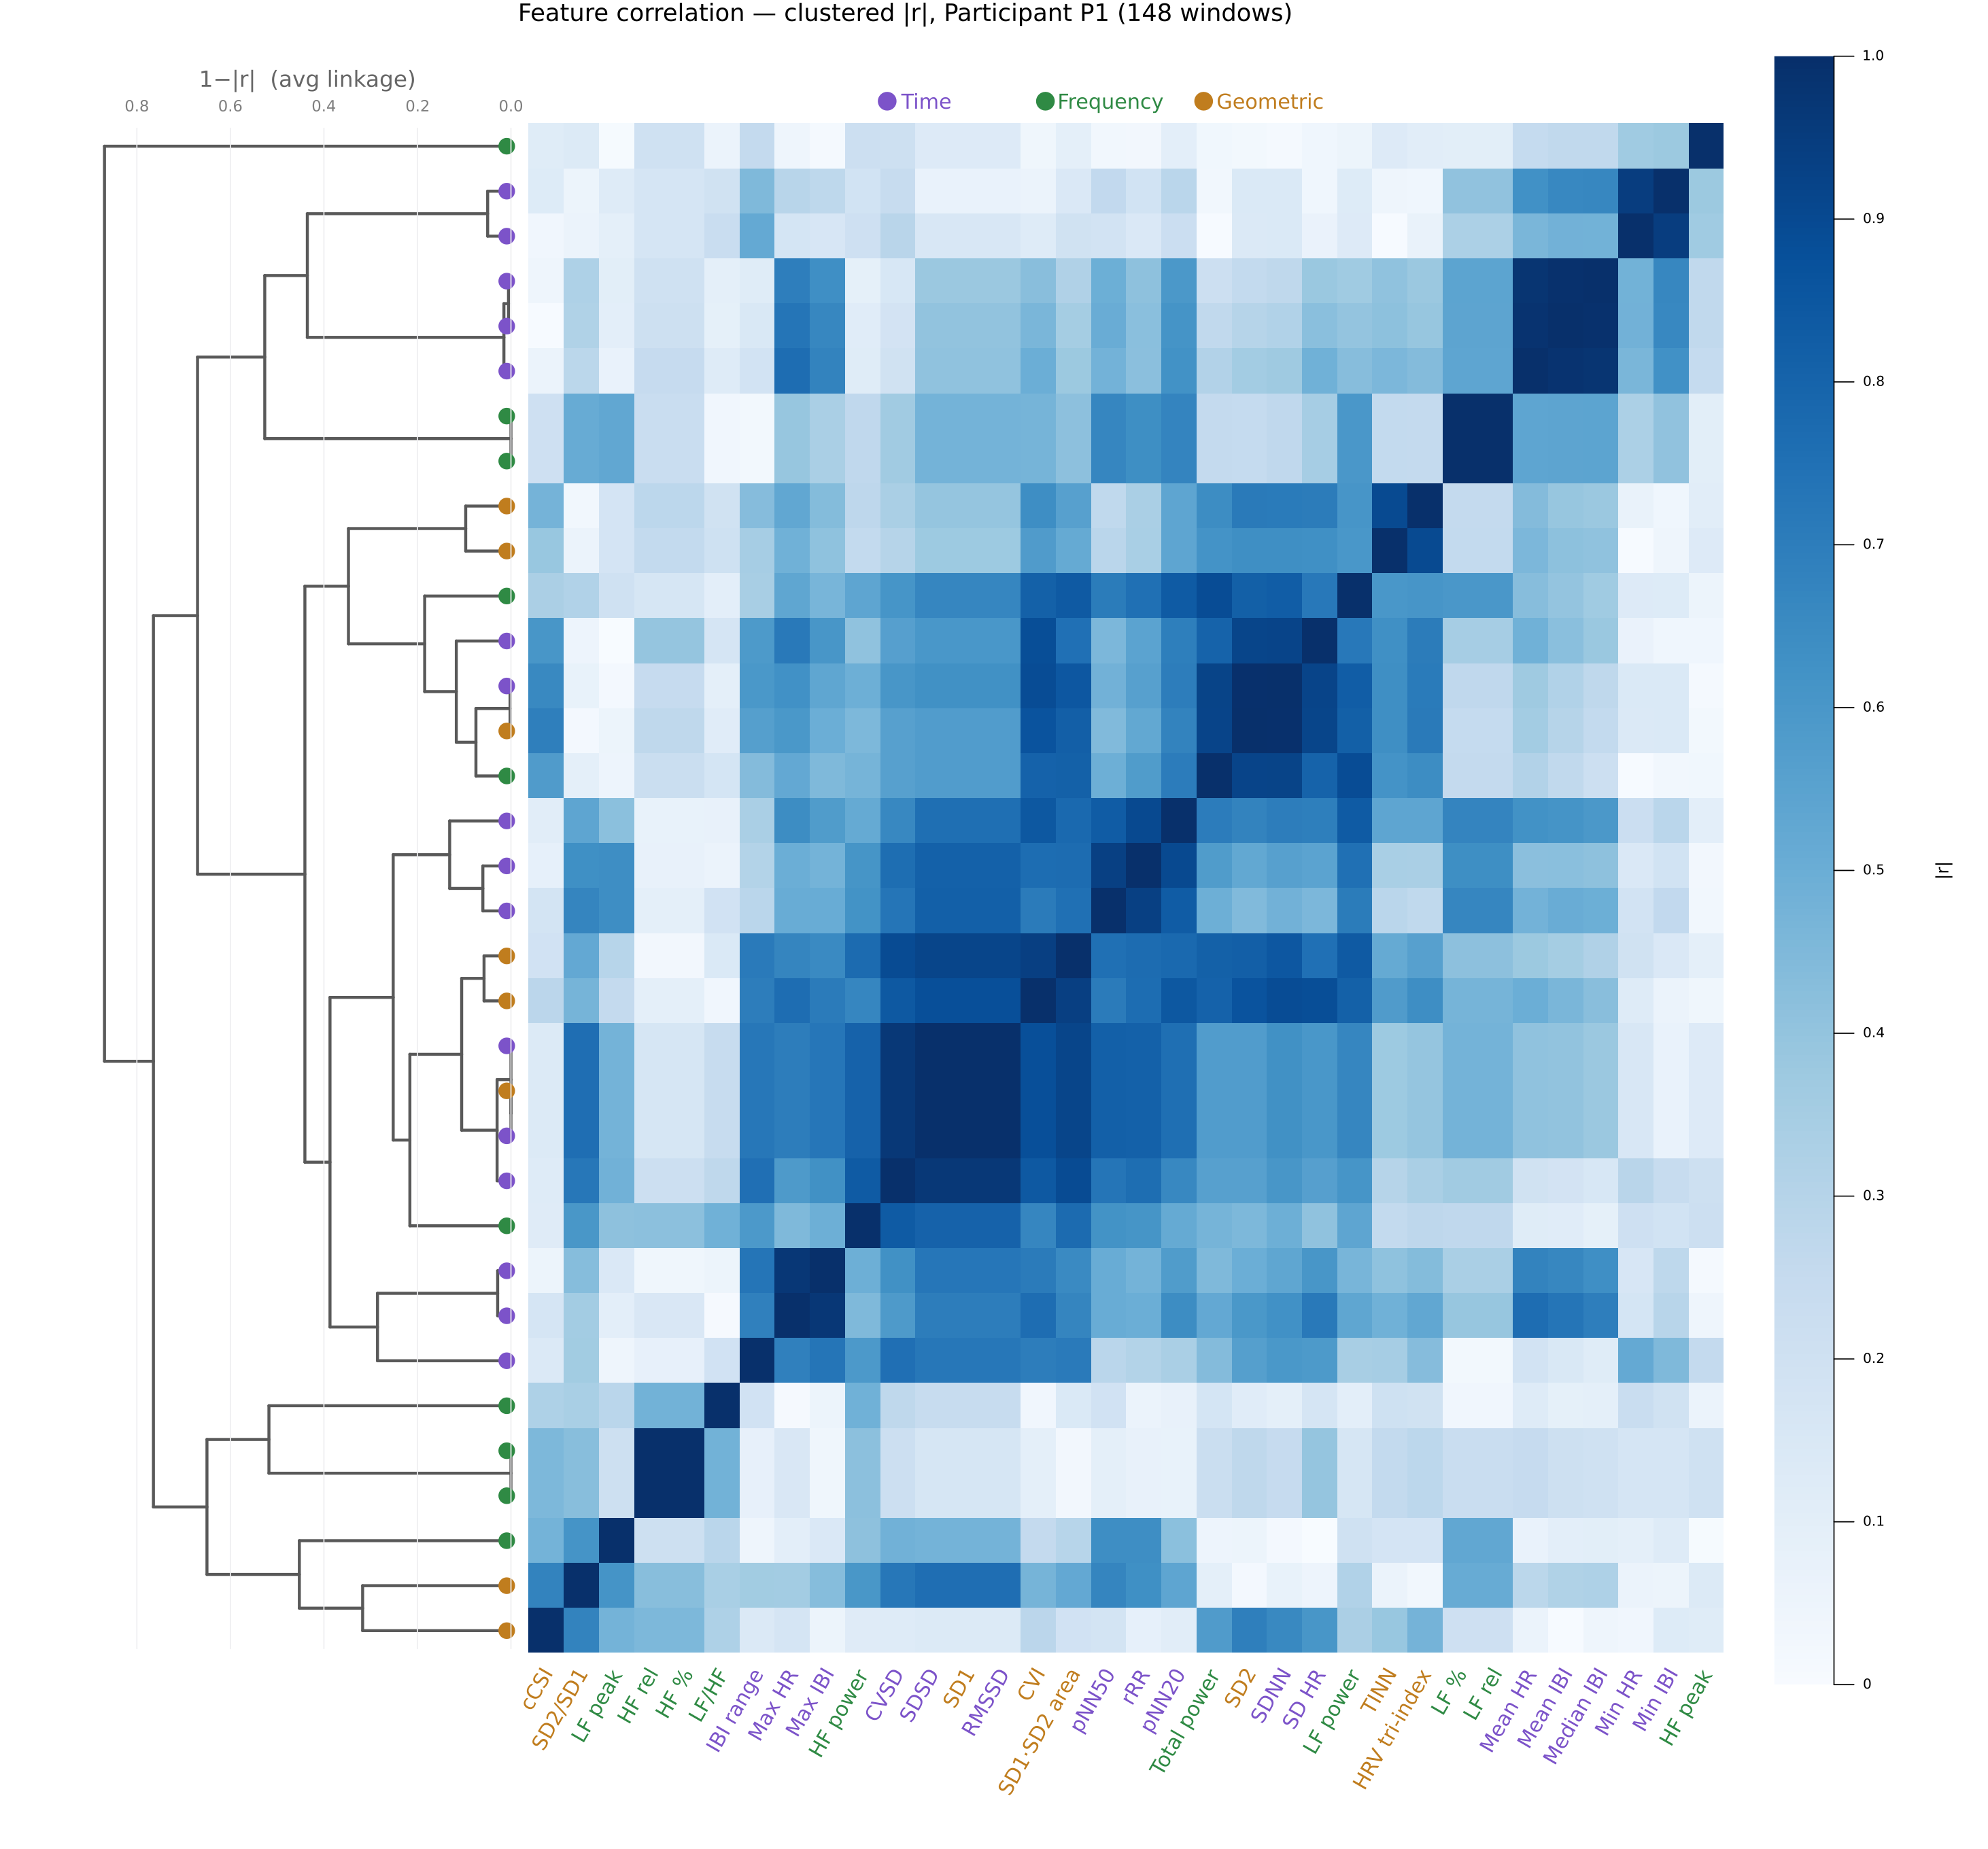
\includegraphics[width=85mm]{figs/p1_correlation.png}\end{center}
  \vspace{0.5mm}
  {\raggedright\footnotesize\color{white!88}
   $|r|$ among features across P1's \textbf{148 windows}, clustered. The same
   near-duplicate blocks the population shows (SD1/RMSSD/SDSD, the LF family) ---
   collinearity is \textbf{structural}, not a dataset artifact.\par}
\end{tcolorbox}%
\end{minipage}%
\foldguides

\end{document}
